\documentclass{article}
\usepackage[utf8]{inputenc}
\usepackage[T1]{fontenc}
\usepackage{graphicx}
\usepackage{grffile}
\usepackage{longtable}
\usepackage{wrapfig}
\usepackage{rotating}
\usepackage[normalem]{ulem}
\usepackage{amsmath}
\usepackage{textcomp}
\usepackage{amssymb}
\usepackage{capt-of}
\usepackage{hyperref}
\author{Carolina Silva, Cristina Pinto, João Fraga}
\date{\today}
\title{Projeto Sistemas Operativos}
\hypersetup{
 pdfauthor={Carolina Silva, Cristina Pinto, João Fraga},
 pdftitle={Projecto Sistemas Operativos},
 pdfkeywords={},
 pdfsubject={},
 pdfcreator={},
 pdflang={English}}

\begin{document}

\maketitle
\tableofcontents

\pagebreak{}
\section{Introdução}
\label{sec:org0490e64}

Este trabalho consiste no desenvolvimento e uma aplicação de linha de comandos destinada a gestão de matriculas de estudantes de Erasmus, na Universidade da Beira Interior, mas que poderia ser adaptado para os restantes estudantes da mesma universidade.

A aplicação e constituída por um conjunto de scripts e ficheiros implementados para dar resposta ao problema abordado.
Recorrendo a comandos de Bash Shell, a aplicação permite a gestão e criação de relatórios, recorrendo a bases de dados com informações das universidades, professores, estudantes e disciplinas.
Pretende ainda implementar um conjunto de funcionalidades, que contemplam Registar, Editar, Eliminar, Consultar, Listar, Relatórios ou Backups com informações estatísticas pertinentes.
Trata-se de uma aplicação constituída por vários menus com o objetivo de a tornar mais pratica para qualquer utilizador.

Como suporte para o desenvolvimento deste trabalho, recorremos aos materiais fornecidos pelo docente da unidade curricular, bem com a bibliografia de referencia sugerida para esta disciplina.

\section{Base de dados}
\label{sec:org6d65565}

A Base de Dados permite armazenar toda a informação referente as varias entidades deste projeto, nomeadamente, a universidade, professores, estudantes e disciplinas.
Cada tabela da base de dados foi estruturada, tendo em conta a informação relevante de cada entidade.

\subsection{Universidades}
\label{sec:orgdba02d4}

\begin{center}
\begin{tabular}{rlrllr}
\hline
ID & Nome & Contacto & Morada & Pais & ETCS\\
\hline
1 & Leeds University & 999999999 & Leeds & UK & 30\\
2 & Universite d'Orleans & 888888888 & Orleans & FR & 30\\
3 & Universidade Federal Rio & 777777777 & Rio Grande & BR & 30\\
\hline
\end{tabular}
\end{center}

\subsection{Professores}
\label{sec:org960cfbe}

\begin{center}
\begin{tabular}{rlrll}
\hline
ID & Nome & Contacto & Universidade & Departamento\\
\hline
1 & William S. & 222222222 & Leeds University & Math\\
2 & Louis Delphine & 333333333 & Universite d'Orleans & Informatique\\
3 & Matheus B. & 444444444 & Universidade Federal Rio & Informatica\\
\hline
\end{tabular}
\end{center}

\pagebreak{}
\subsection{Estudantes}
\label{sec:org1d4e9d4}

\begin{center}
\begin{tabular}{llllllp{1.5cm}p{1.7cm}}
\hline
ID & Nome & Contacto & Universidade & Curso & Professor & Numero \newline Disciplinas & Lista \newline Disciplinas\\
\hline
1 & Charles & 930000000 & 1 & E.I. & 1 & 5 & 1, 2, 3, 4, 5\\
2 & Anne & 930000000 & 2 & E.I. & 2 & 4 & 1, 3, 4, 5\\
3 & Joao & 930000000 & 3 & E.I. & 3 & 3 & 1, 3, 4\\
\hline
\end{tabular}
\end{center}

\subsection{Disciplinas}
\label{sec:org7da50e0}

\begin{center}
\begin{tabular}{rlrrlr}
\hline
ID & Nome & Ano & Semestre & Regente & Creditos\\
\hline
1 & Sistemas Operativos & 2 & 2 & Paul Crocker & 6\\
2 & Base de Dados & 2 & 2 & Joao Muranho & 6\\
3 & Teoria da Computação & 2 & 2 & Simao Sousa & 6\\
4 & Engenharia de Software & 2 & 2 & Nuno Pombo & 6\\
5 & Tecnologias Multimedia & 2 & 2 & Valderi Leithardt & 6\\
\hline
\end{tabular}
\end{center}

\section{Ficheiros}
\label{sec:org338e199}

Todas as informações criadas nesta aplicação são armazenadas em diversos ficheiros, associados a cada entidade (universidade, professores, estudantes e disciplinas), com a extensão .csv.

No caso dos backups, estes são armazenados em ficheiros comprimidos, com a extensão .tar.gz, que poderão ser posteriormente restaurados, a partir de uma determinada data ou ponto de restauro selecionado pelo utilizador.

\vspace{1cm}

Pasta backup:

\begin{itemize}
\item backup/user/date1.tar.gz
\item backup/user/date2.tar.gz
\item backup/user/date3.tar.gz
\end{itemize}

\vspace{1cm}

Pasta data:

\begin{itemize}
\item data/universidades.csv
\item data/professores.csv
\item data/estudantes.csv
\item data/disciplinas.csv
\end{itemize}

\pagebreak{}
\section{Menus}
\label{sec:org7cc711f}

A aplicação desenvolvida e constituída por um conjunto de menus com o objetivo de facilitar a interação com o utilizador.

\vspace{2cm}

\begin{figure}[h]
\centering
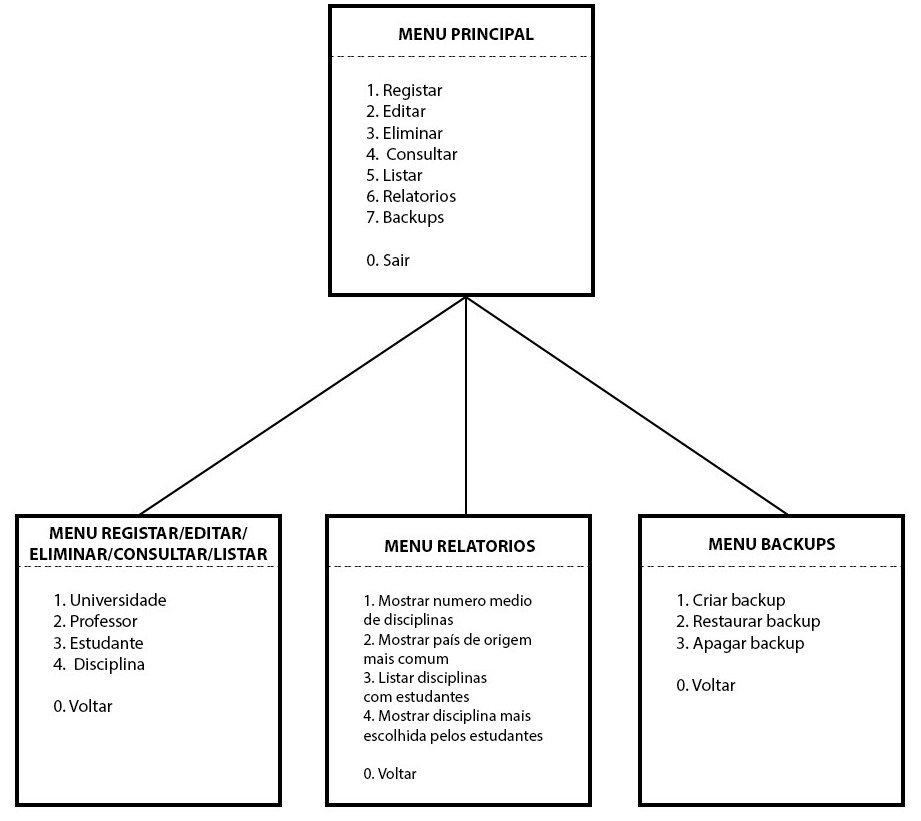
\includegraphics[scale=0.4]{images/esquema}
\caption{Esquema de menus}
\end{figure}

\pagebreak{}
\section{Programas}
\label{sec:orge1cc32e}

Para facilitar a interação da aplicação com o utilizador foram desenvolvidos um conjunto de programas.

Assim, foi desenvolvido um programa principal onde estão enumeradas todas as funcionalidades da aplicação, nomeadamente, registar, editar, eliminar, consultar, listar, relatório, backup e sair.

\subsection{main.sh}
\label{sec:org5bbb6c0}

main.sh e um programa que trata de inicializar a estrutura em pastas inicial e redirecionar o utilizador para os submenus apropriados tendo em conta a sua opção.

\begin{figure}[h]
\centering
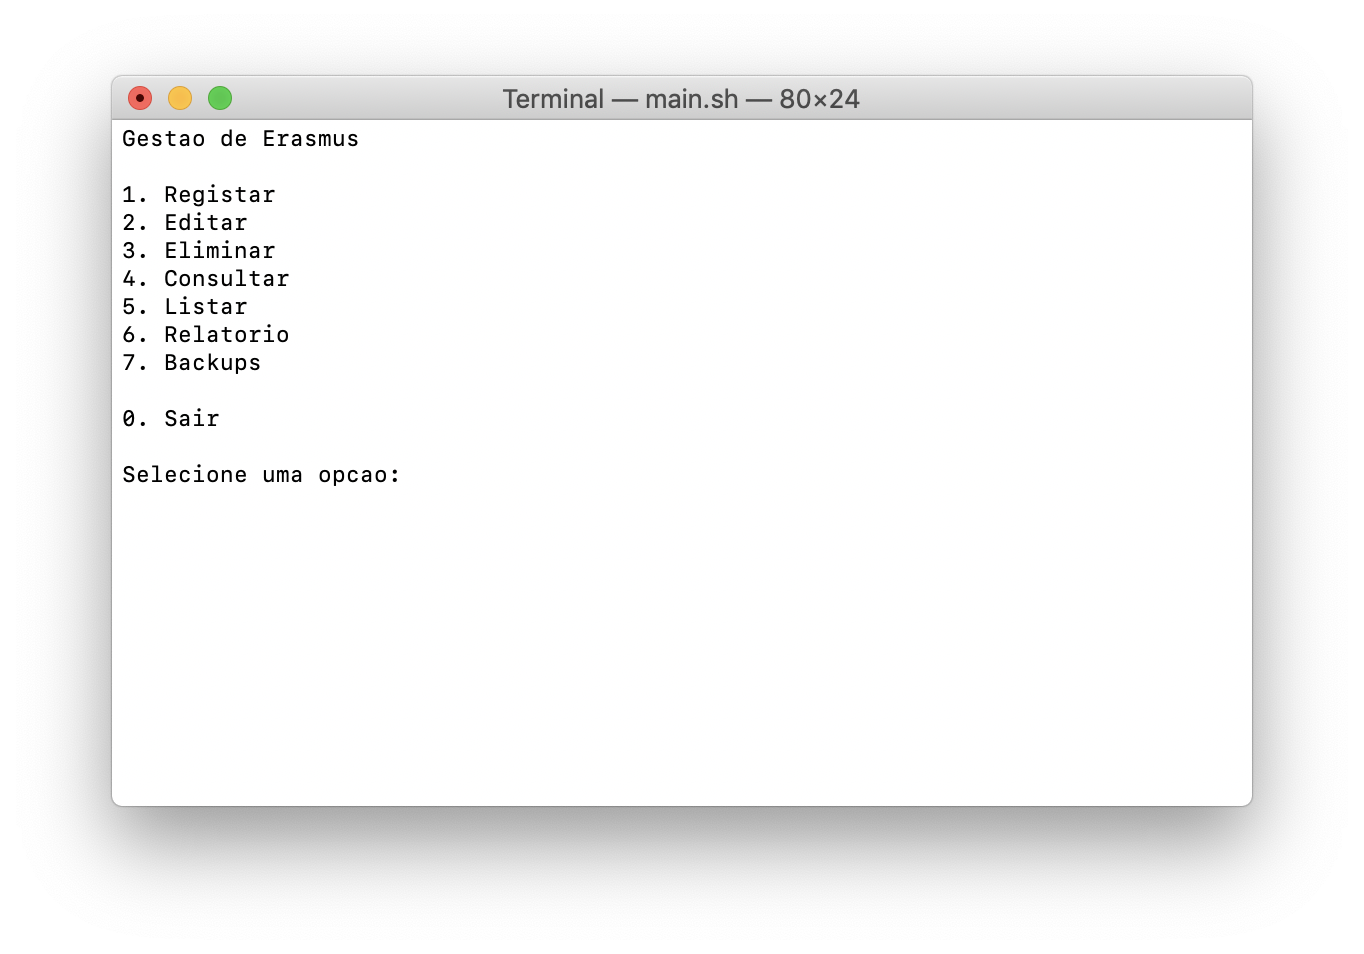
\includegraphics[scale=0.4]{images/MainMenu}
\caption{Menu principal}
\end{figure}

Comandos utilizados:

\begin{itemize}
\item echo - apresentar informação
\item read - pedir input
\item mkdir - criar directorias
\end{itemize}

\pagebreak{}
\subsection{registar.sh}
\label{sec:org3ac8dd4}

registar.sh e um programa que trata da implementação da funcionalidade de registo de novas entidades.
Permite ao utilizador registar uma universidade, um(a) professor(a), um estudante ou uma disciplinas.

\begin{figure}[h]
\centering
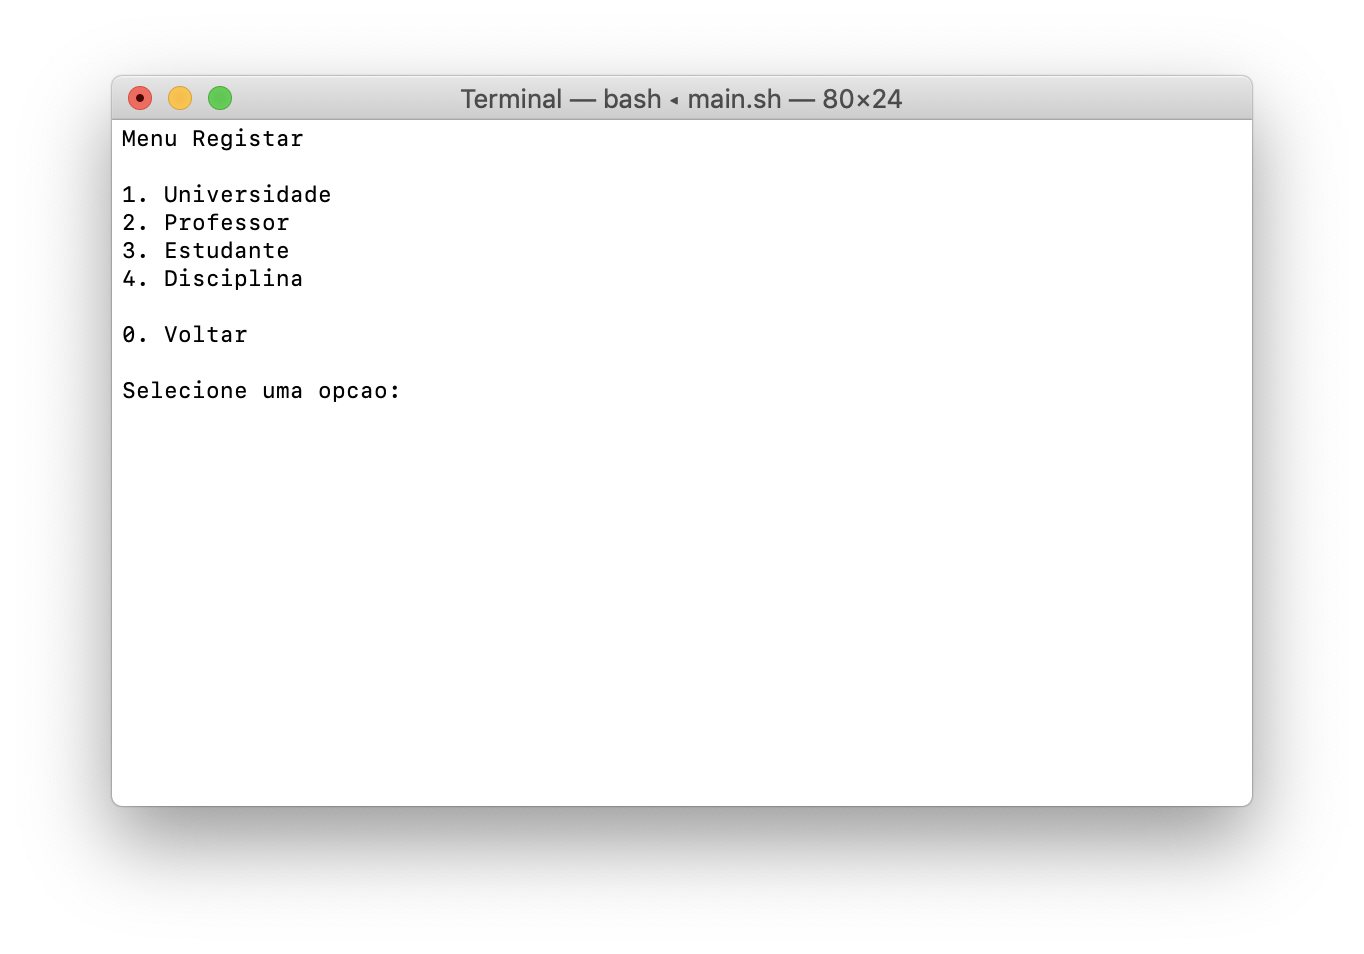
\includegraphics[scale=0.4]{images/MenuRegistar}
\caption{Menu registar}
\end{figure}

Comandos utilizados:

\begin{itemize}
\item echo - apresentar informação / adicionar informação a ficheiros
\item read - pedir input
\end{itemize}

\pagebreak{}
\subsection{editar.sh}
\label{sec:orgd7c4c66}

editar.sh e um programa que trata da implementação da funcionalidade de edição de um registo.
Permite ao utilizador alterar a informação de uma universidade, professor(a), estudante ou disciplina.

\begin{figure}[h]
\centering
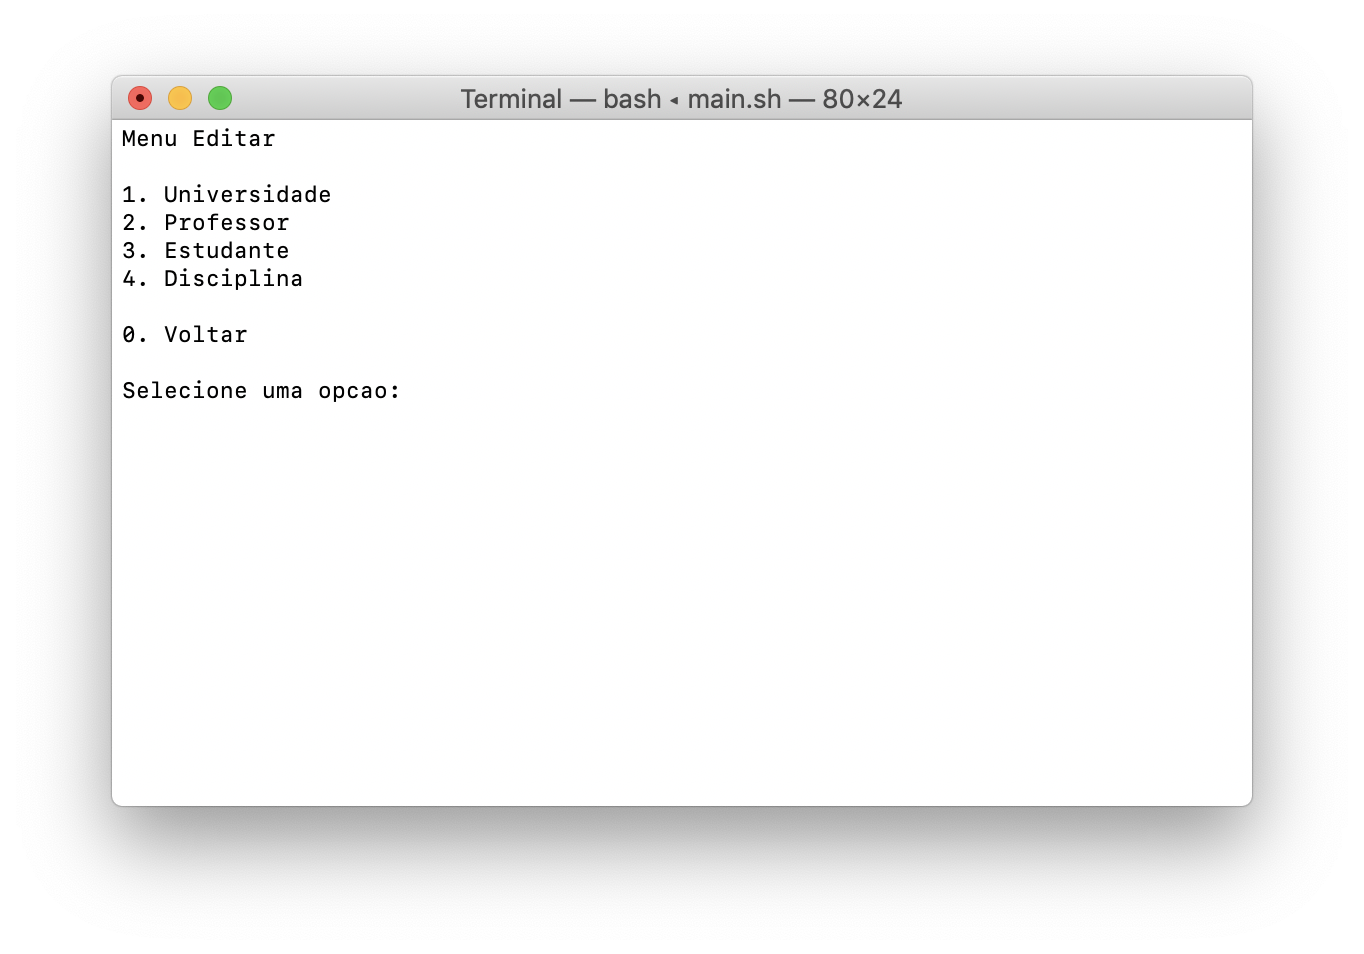
\includegraphics[scale=0.4]{images/MenuEditar}
\caption{Menu editar}
\end{figure}

Comandos utilizados:

\begin{itemize}
\item echo - apresentar informação
\item read - pedir input
\item awk - selecionar linha ficheiro
\item cut - obter informação de uma coluna
\item sed - substituir informação do ficheiro
\end{itemize}

\pagebreak{}
\subsection{eliminar.sh}
\label{sec:org608b6d0}

eliminar.sh e um programa que trata da implementação da funcionalidade de eliminar um registo.
Permite ao utilizador eliminar uma universidade, um(a) professor(a), um estudante ou uma disciplina, através de uma pesquisa por “ID” ou por “nome”.

\begin{figure}[h]
\centering
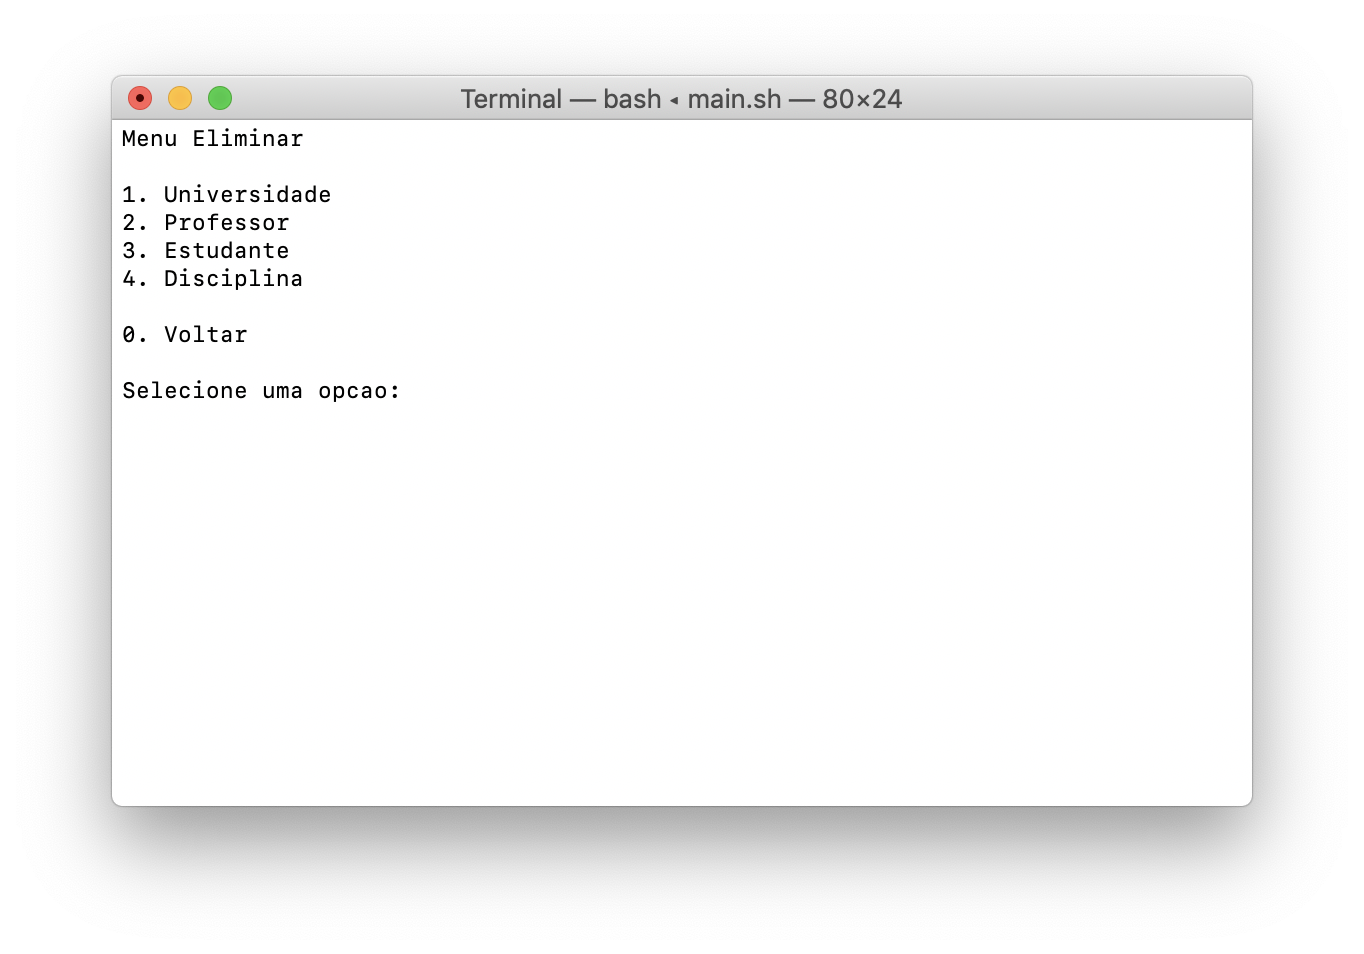
\includegraphics[scale=0.4]{images/MenuEliminar}
\caption{Menu eliminar}
\end{figure}

Comandos utilizados:

\begin{itemize}
\item echo - apresentar informação
\item read - pedir input
\item awk - selecionar entidade
\item cat - criar/imprimir conteúdo ficheiro
\end{itemize}

\pagebreak{}
\subsection{consultar.sh}
\label{sec:orgd2facc6}

consultar.sh e um programa que trate de apresentar informações sobre uma entidade especifica.
Permite ao utilizador procurar uma universidade, professor(a), estudante, disciplina.

\begin{figure}[h]
\centering
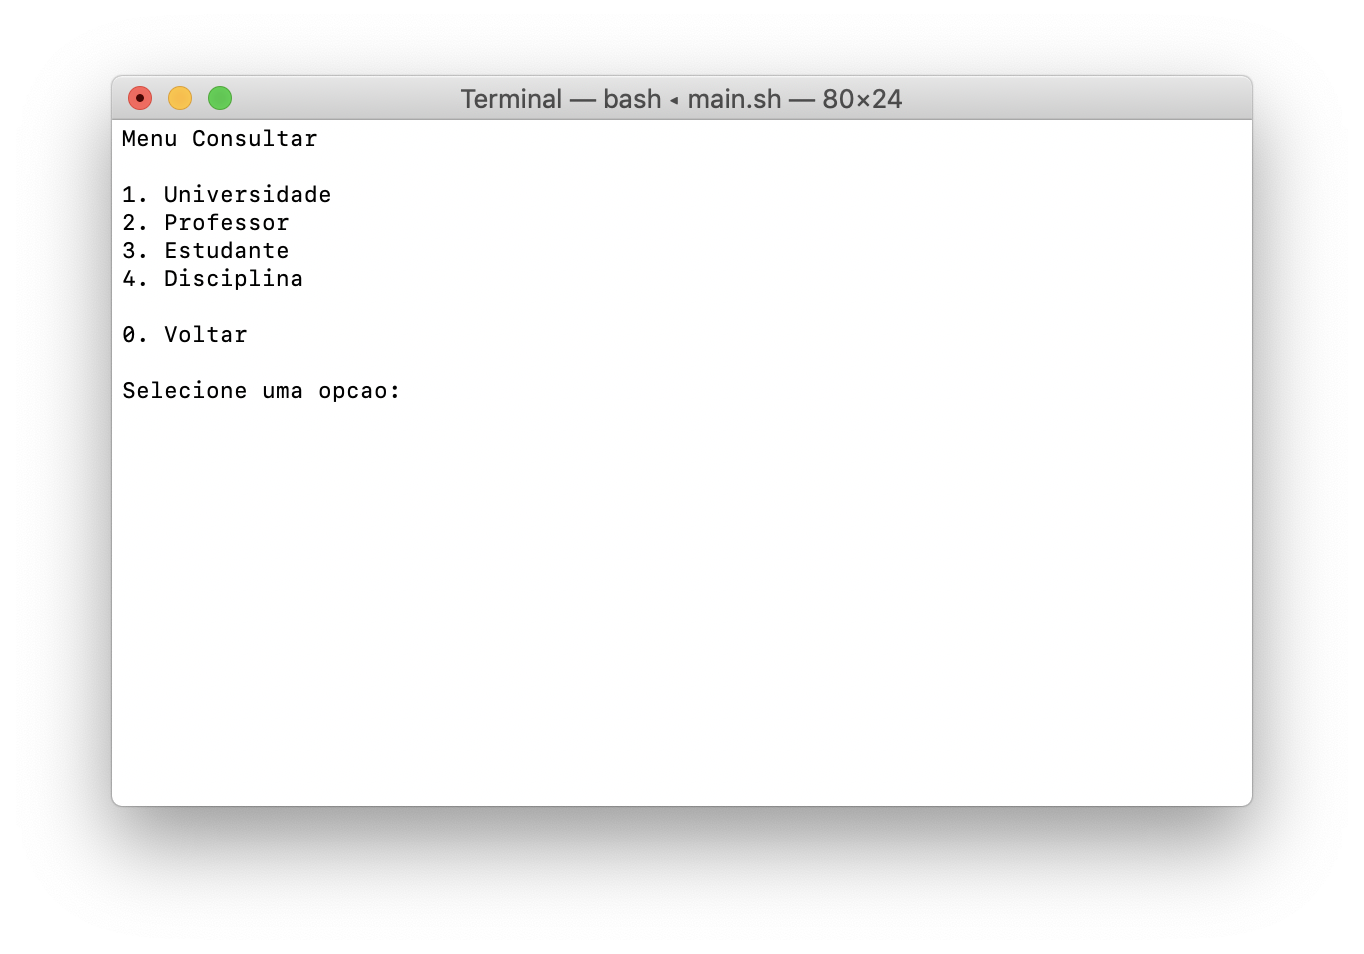
\includegraphics[scale=0.4]{images/MenuConsultar}
\caption{Menu consultar}
\end{figure}

Comandos utilizados:

\begin{itemize}
\item echo - apresentar informação
\item read - pedir input
\item awk - selecionar entidade
\end{itemize}

\pagebreak{}
\subsection{listar.sh}
\label{sec:org4ba6c40}

listar.sh e um programa que trata da apresentação de toda a informação das varias entidades.
Permite apresentar uma lista de todas as universidades, professores, estudantes ou disciplinas registadas anteriormente.

\begin{figure}[h]
\centering
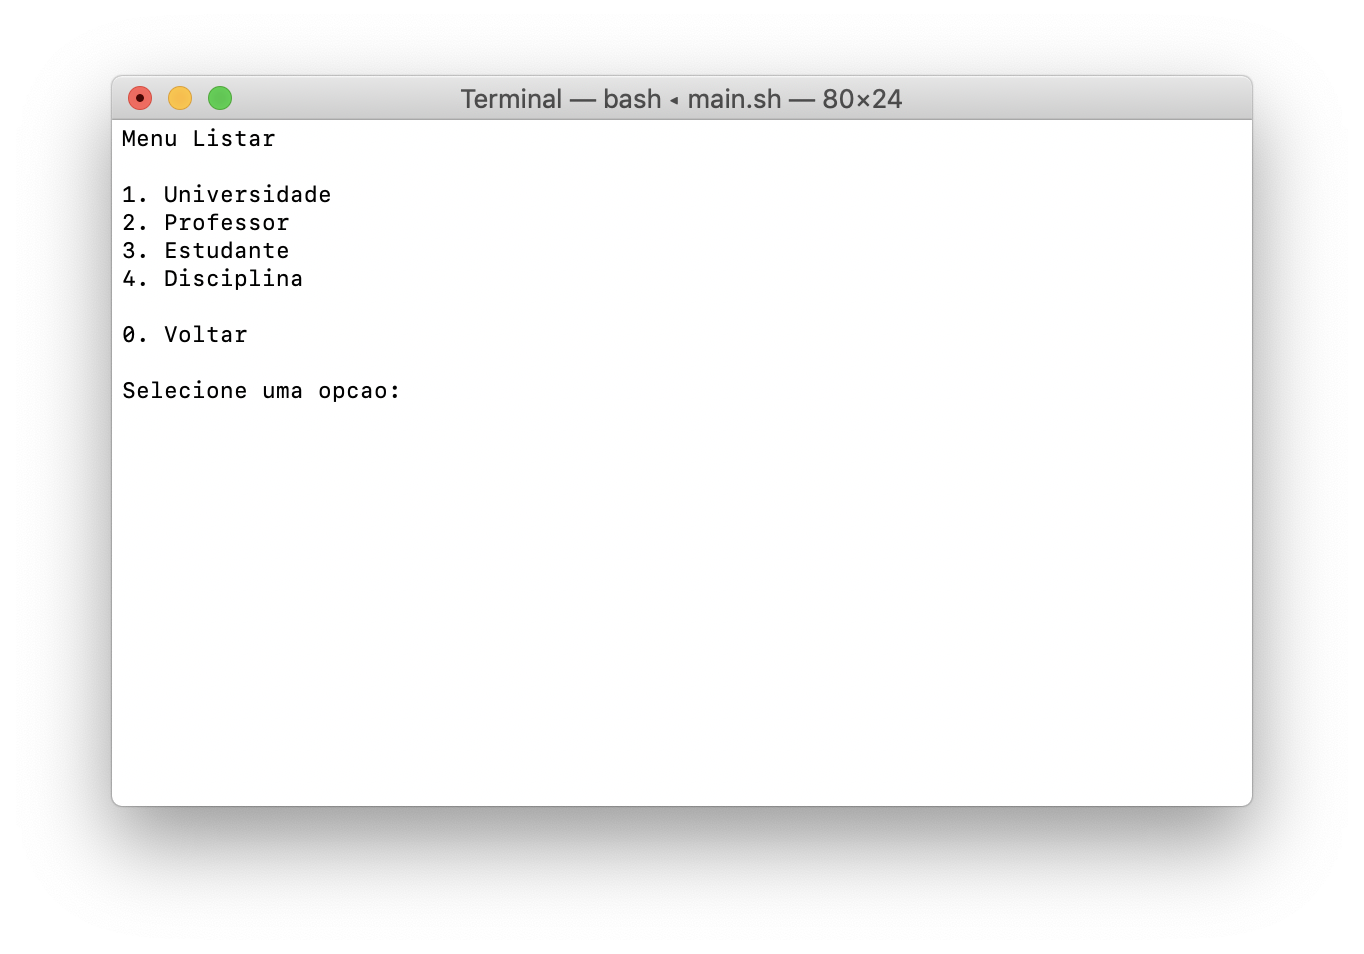
\includegraphics[scale=0.4]{images/MenuListar}
\caption{Menu listar}
\end{figure}

Comandos utilizados:

\begin{itemize}
\item echo - apresentar informação
\item read - pedir input
\item cat - criar/imprimir conteúdo ficheiro
\end{itemize}

\pagebreak{}
\subsection{relatorios.sh}
\label{sec:org28d85c0}

relatorio.sh e um programa que trata do calculo e apresentação de varias estatísticas.
Permite ao utilizador consultar qual o numero medio de disciplinas a que um aluno de Erasmus esta inscrito, qual pais de origem mais comum, quais as disciplinas com estudantes inscritos e quais destas são as mais populares entre os estudantes.

\begin{figure}[h]
\centering
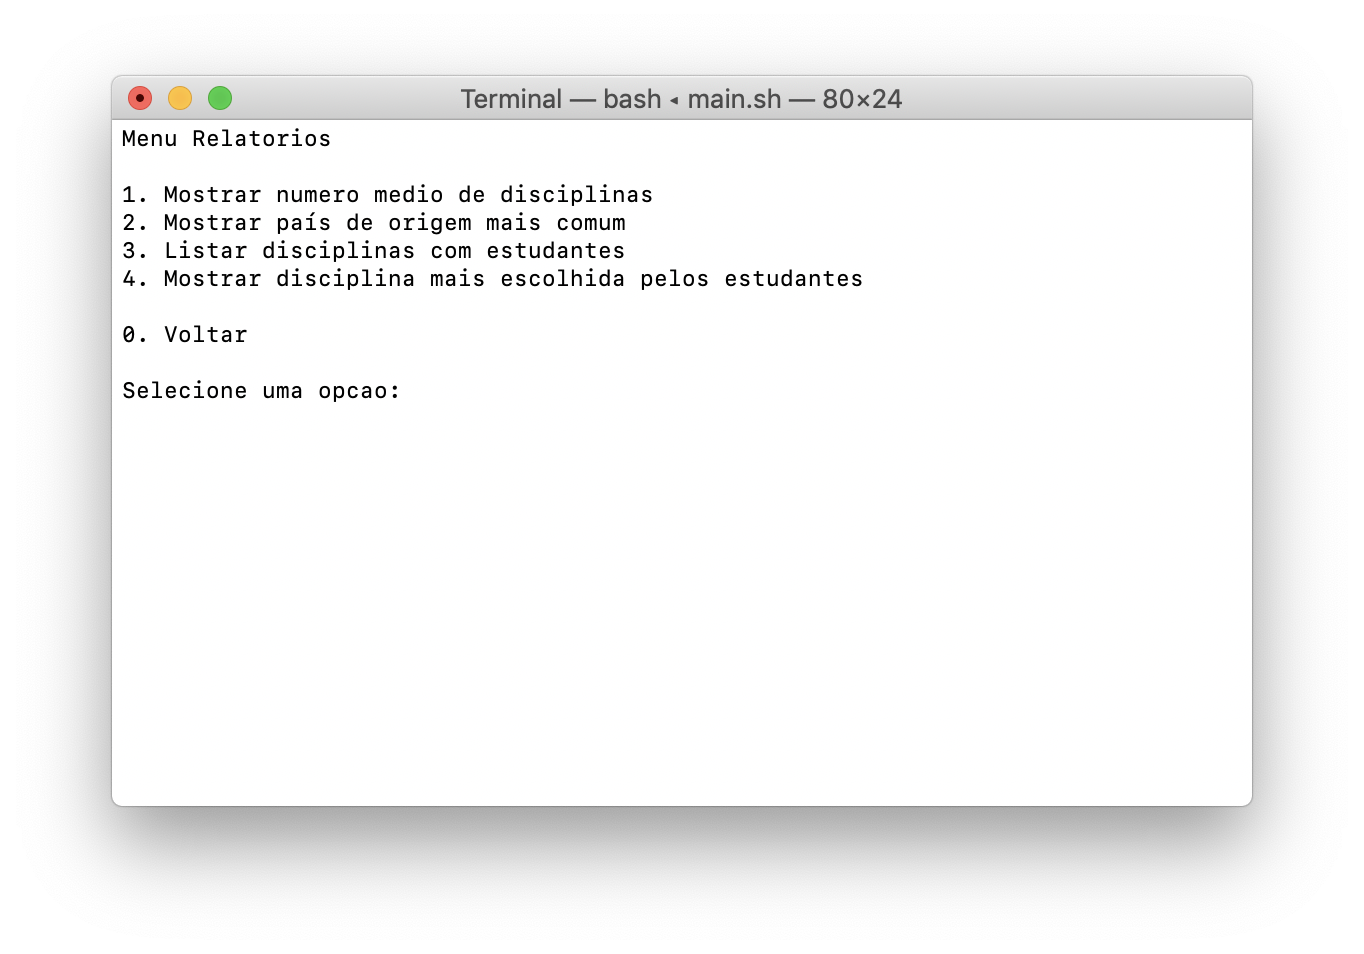
\includegraphics[scale=0.4]{images/MenuRelatorios}
\caption{Menu relatorios}
\end{figure}

Comandos utilizados:

\begin{itemize}
\item wc - contar linhas do ficheiro
\item seq - obter sequencia de números
\item head/tail - selecionar linha
\item cut - obter informação de uma coluna
\item echo - apresentar informação
\item read - pedir input
\item cat - criar/imprimir conteúdo do ficheiro
\item awk - selecionar linha do ficheiro
\item sort - ordenar ficheiro
\item uniq - eliminar linhas iguais adjacentes
\end{itemize}

\pagebreak{}
\subsection{backup.sh}
\label{sec:org6ed11a5}

backup.sh e um programa que trata da implementação de toda a funcionalidade de backup.
Permite ao utilizador criar/eliminar backups que estão armazenados na pasta backup.
E possível também restaurar um backup através de uma lista de backups que é gerada com base nos backups presentes na pasta backup

\begin{figure}[h]
\centering
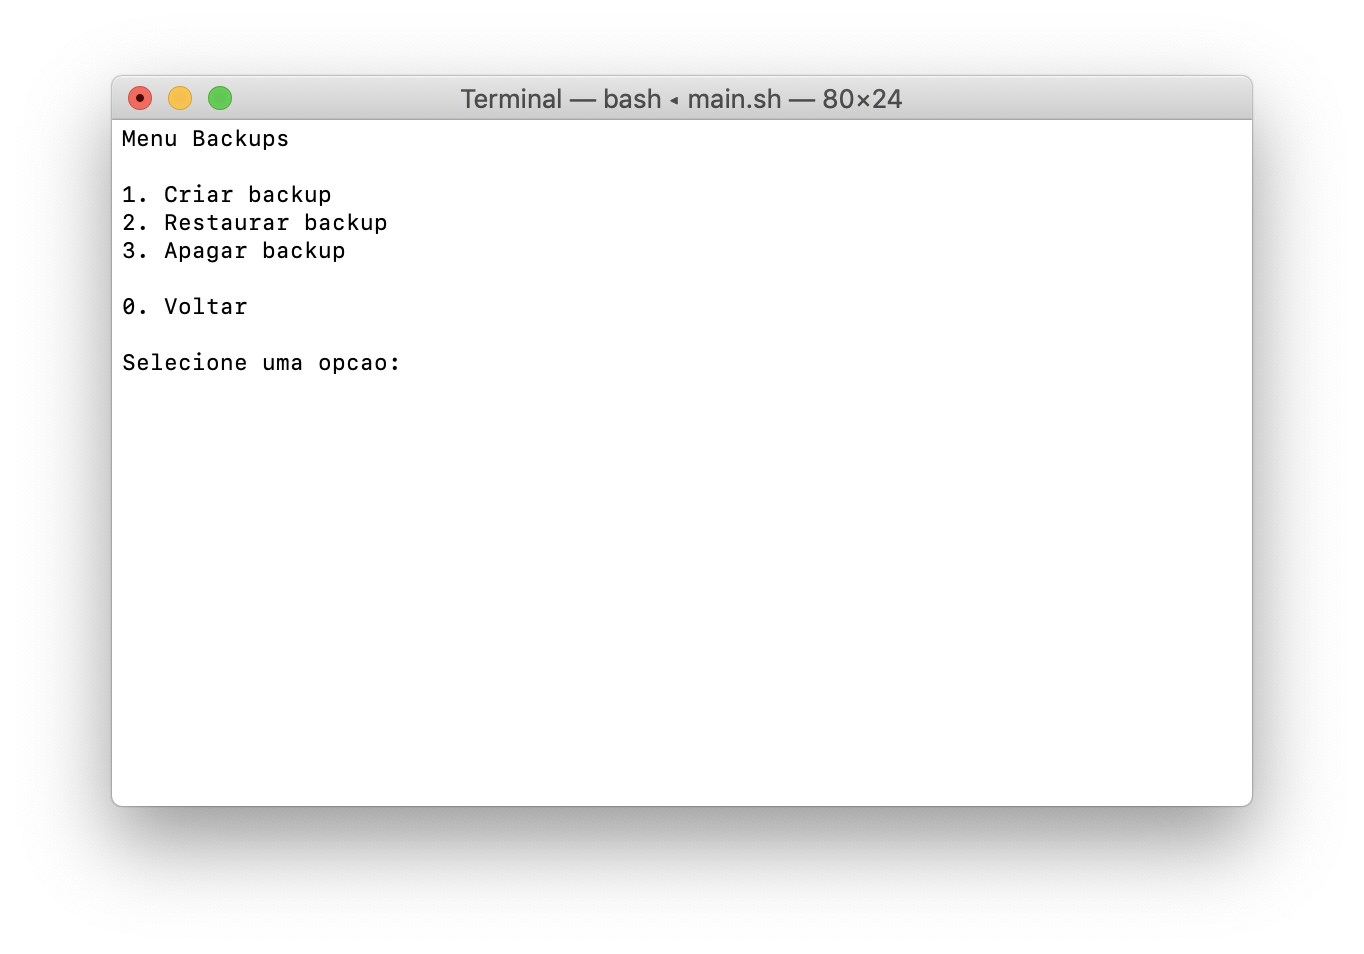
\includegraphics[scale=0.4]{images/MenuBackups}
\caption{Menu backups}
\end{figure}

Comandos utilizados:

\begin{itemize}
\item echo - apresentar informação
\item read - pedir input
\item tar - comprimir backups
\item nl - numerar backups
\item rm - remover backups
\item find - encontrar backups
\item sed - selecionar linha
\end{itemize}

\end{document}
